\documentclass[12pt,english]{scrartcl}

\usepackage{amsmath,amssymb}
%\usepackage[amssymb]{SIunits}
\usepackage{babel}
\usepackage[latin1]{inputenc}
\usepackage{graphicx}
\usepackage{color}
\usepackage{url}


\begin{document}

\begin{center}
\textbf{\begin{LARGE}KOGW-PM-KNP:\\ \vspace{3mm} Tutorial 7 - Central Interference in Driving
\end{LARGE}}
\end{center}

This tutorial deals with an applied research question namely to what extent an automated task like driving is subject to interference from a secondary task. Please read the paper carefully. Answer the following questions which should help you to evaluate their findings. Please work in pairs. 
%  
% \begin{figure}[htbp]
% \begin{center}
% 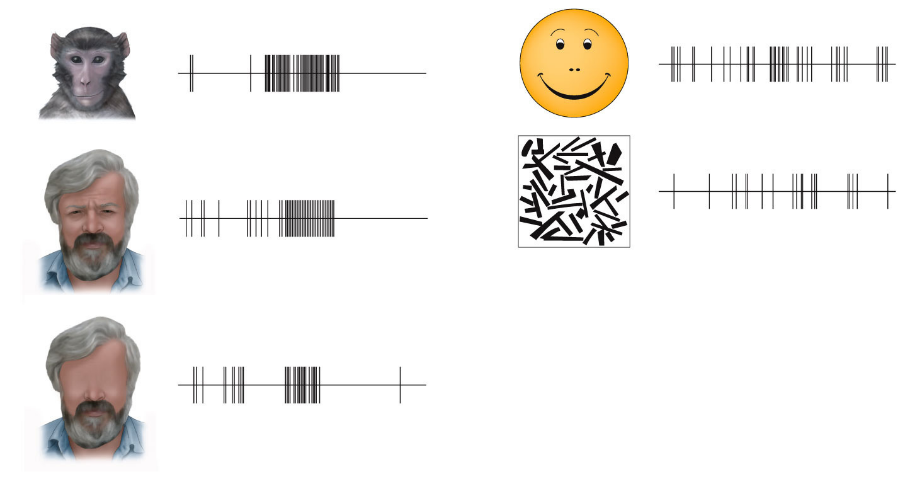
\includegraphics[width = 0.8\textwidth]{IT_cell.png}
% \end{center}
% \caption{
% \label{fig:IT_cell}}
% \end{figure}

\begin{enumerate}
 \item What does the \textit{central-bottleneck} hypothesis say? What kind of evidence supports the hypothesis? Think of an effect that we discussed in the lecture that is an example of the psychological refractory period.

 \color{blue}
 \begin{itemize}
 \item certain mental operations cannot be performed in parallel because they employ the same central ressources
 \item for responses to two stimuli that are presented in rapid succession the response to the latter stimulus is slowed down for short SOAs
 \item attentional blink effect - RVSP
 \end{itemize}
  \color{black}

 \item Name the reasons why people think that bottleneck-type delays might not apply to real-world activities.

  \color{blue}
 \begin{itemize}
 \item conditions too different from realistic ones: punctuate stimuli, predictable order, separated by SOA, speeded response ...
\item real-world tasks much more practiced
 \end{itemize}
  \color{black}

\item What was the goal of the present study and how was it realized?

\color{blue}
 \begin{itemize}
 \item Test whether CB phenomena generalize to real-world activity of driving
 \item driving simulator - years of experience with driving - still PRP effect?
 \item participants followed a lead car
 \item task 1: \textit{braking task}
 \item task 2: intermittent choice response task: visual or auditory stimulus presented once or twice $\rightarrow$ manual or vocal response
 \item SOA variation
 \end{itemize}
  \color{black}

 \item CB phenomena are typically found for choice response tasks (CRT). The authors argue that although the braking task is rather similar to a simple reaction time task (SRT) they nevertheless expect interference. What are their arguments and do you follow their reasoning?

\color{blue}
 \begin{itemize}
 \item SRT: brake light $\rightarrow$ depress brake pedal
 \item effector (right foot) not on brake pedal
 \item entertain various options when braking - decision making
 \end{itemize}
  \color{black}


\item Which factors were manipulated by the experimenters?
\color{blue}
 \begin{itemize}
 \item modality of stimulus presentation: visual (rear window turns white) or auditory (400Hz tone)
 \item modality of response: vocal (``one'', ``two''), manual (one, two button presses) - between blocks
 \item SOA: 0, 150, 350, 1200ms, within blocks
 \item single-task trials: choice or braking (16 each)
 \item dual-task trials: (8)
 \end{itemize}
  \color{black}


\item What were the main results of the study?
\color{blue}
Choice task
 \begin{itemize}
 \item single task: main effects of both stimulus and response modality
 \item dual task: main effects + interaction
 \item no effect of SOA on single tasks: choice and brake, nor much on choice dual task 
 \end{itemize}
brake task 
 \begin{itemize}
 \item braking response is markedly slowed down by concurrent choice task: RT decreased with increasing SOA = PRP effect
 \item gas-off RT: lights off until gas pedal is deflected by 20\%
 \item movement RT: remaining portion of brake RT
 \end{itemize}
  \color{black}

\item What do the authors conclude from the present results? Do you agree?
  \color{blue}
\begin{itemize}
 \item PRP/dual task interference generalizes to highly practiced, real-world task $\Rightarrow$ vehicle braking is \textbf{not} automatic
 \item effect of SOA on brake RT ($RT_{350} - RT_{0}$) produced delay of 174ms: 5m difference for a car travelling at 100km/h 
 \item PRP can be observed even for a task that resembles a laboratory SRT, real-word driving likely more complex
 \item single-task trials evenly split between the tasks - equal priority to both tasks (?)
 \item mainly gas-off RTs affected: dual-task slowing occurred prior to reponse initiation, response planning not motor control 
 \item performing a concurrent task can seriously impair driving even when the tasks do not overlap in their sensory or response modalities
 \end{itemize}
  \color{black}

\item Why did the authors perform the follow-up experiment? How did it differ from the main experiment? What were the results?
\color{blue}
 \begin{itemize}
 \item test the generalizability of their primary finding
 \item no driving, stimulus was gray rectangle upper half flashed white $\rightarrow$, brake stimulus: rectangle with two circles that were black but became red, depress gas pedal except when executing a braking response 
 \item similar results
 \end{itemize}
  \color{black}

\end{enumerate}
\end{document}
